\chapter{Efficient Algorithm Selection}
\label{chapter:alphalinkage}

We define $\alpha$ as the parameter with which the distance of an algorithm is weighted. In this chapter we propose different distance measurements depending on the weight parameter $\alpha$ that allow us to interpolate between different linkage strategies in a way similar to the proposed by Balcan et al. \cite{DBLP:journals/corr/BalcanNVW16}, where an infinite interval was introduced.\\

To be able to solve the mathematical problem, we need to have a finite set of intervals. So we interpolate between one algorithm with $\alpha = 0$ and another algorithm with $\alpha = 1$, where for $\alpha = 0$ the result will be the result of algorithm 1 and for $\alpha = 1$ the result of algorithm 2. For instance for $\alpha = 0.5$, we will weight the outputs of both algorithms equally, i.e.\ distance $D = 0.5 \cdot D_1 + 0.5 \cdot D_2$.

\section{Linear Interpolation Between Two Different Linkage Strategies}

Interpolating between two of the three mentioned linkage strategies results in three different algorithmic settings. In the first setting we are using the single linkage distance $d_{SL}(X,Y)$ and the complete linkage distance $d_{CL}(X,Y)$. By combining the two distances we can create a linear model that ranges from $\alpha = 0$ (single linkage) to $\alpha = 1$ (complete linkage) resulting in equation \ref{eq:singlecomplete}.

\begin{equation}
    \begin{aligned}
        \dsc(X,Y,\alpha) &= (1 - \alpha) \cdot d_{SL}(X,Y) + \alpha \cdot d_{CL}(X,Y)\\
        &= (1 - \alpha) \min\limits_{x \in X, y \in Y} d(x,y) + \alpha \max\limits_{x \in X, y \in Y} d(x,y)
    \end{aligned}
    \label{eq:singlecomplete}
\end{equation}

Equivalently, we can interpolate between the single linkage distance $d_{SL}(X,Y)$ and the average linkage distance $d_{AL}(X,Y)$ instead of the complete linkage distance $d_{CL}(X,Y)$ for $\alpha = 1$ resulting in equation \ref{eq:singleaverage}. 

\begin{equation}
    \begin{aligned}
        \dsa(X,Y,\alpha) &= (1 - \alpha) \cdot d_{SL}(X,Y) + \alpha \cdot d_{AL}(X,Y)\\
        &= (1 - \alpha) \min\limits_{x \in X, y \in Y} d(x,y) + \alpha \frac{1}{|X| |Y|}\sum\limits_{x \in X, y \in Y} d(x,y)
    \end{aligned}
    \label{eq:singleaverage}
\end{equation}

The last of the three settings describes the interpolation between the average linkage distance $d_{AL}(X,Y)$ and the complete linkage distance $d_{CL}(X,Y)$ resulting in equation \ref{eq:averagecomplete}.

\begin{equation}
    \begin{aligned}
        \dac(X,Y,\alpha) &= (1 - \alpha) \cdot d_{AL}(X,Y) + \alpha \cdot d_{CL}(X,Y)\\
        &= (1 - \alpha) \frac{1}{|X| |Y|}\sum\limits_{x \in X, y \in Y} d(x,y) + \alpha \max\limits_{x \in X, y \in Y} d(x,y)
    \end{aligned}
    \label{eq:averagecomplete}
\end{equation}

% \section{Linear Interpolation between three different linkage strategies}

\section{Proposed Algorithms}

Our goal is to find an algorithm that finds all different behaviors depending on the value of $\alpha$. To do so, we propose different algorithms. In general, we evaluate results for a data domain $\cX$. Here, we maximize the utility $u$ of a clustering instance with the set of points $S = \{x_1, ..., x_n\} \in \mathcal{X}$ and an (unknown) target clustering $\target = \{C_1, ..., C_k\}$. The output of the bottom up clustering is a binary cluster tree as shown in figure \ref{fig:linkage_effects} and calculated with algorithm \ref{alg:alphalinkage} where the top level node contains one cluster with all points and the leaf nodes contain one cluster for each point. We then prune the cluster tree to $k$ clusters in order to compare these clusters to the target distribution. Afterwards, we use the in section \ref{chapter:costfunctions} discussed cost functions as quality criteria for the resulting criteria.

\begin{algorithm}
\textbf{Input:} Merge functions $\DZero$ and $\DOne$, parameter $\alpha \in [0,1]$, and clustering instance $S = \{x_1, \dots, x_n\}$.
\begin{enumerate}[nosep, leftmargin=*]
\item Let $\mathcal{N} = \{\leaf(x_1), \dots, \leaf(x_n)\}$ be the initial set of nodes (one leaf per point).
\item While $|\mathcal{N}| > 1$
\begin{enumerate}[nosep, leftmargin=*]
  \item Let $A, B \in \mathcal{N}$ be the clusters in $\mathcal{N}$ minimizing $\Dalpha(A,B) = (1-\alpha)\cdot \DZero(A,B) + \alpha \cdot \DOne(A,B)$.
  \item Remove nodes $A$ and $B$ from $\mathcal{N}$ and add $\node(A,B)$ to $\mathcal{N}$.
\end{enumerate}
\item Return the cluster tree (the only element of $\mathcal{N}$).
\end{enumerate}
\caption{$\alpha$-linkage Clustering}
\label{alg:alphalinkage}
\end{algorithm}

 Next, we show an algorithm to divide the interval of $\alpha \in [\alpha_{lo}, \alpha_{hi}]$ into subintervals where the behavior is consistent within each interval, i.e.\ we split the interval $\alpha \in [\alpha_{lo}, \alpha_{hi}]$ into several different executions depending on the parameter $\alpha$. First, we introduce the definition of an execution tree that stores all intervals $\mathcal{I} \in [0,1]$ that lead to different clusterings. We start with the entire range $[\alo, \ahi]$ and then iteratively bound the interval depending on the different merges. The result is a tree where each node represents a different merging behavior (see figure \ref{fig:toe}) and in the end, each leaf node corresponds to one cluster tree.

 \begin{figure}[h]
    \centering
    \includegraphics[width=0.6\textwidth]{images/ClusterTreeFigure}
    \caption{The ``tree of executions'' stores all different merge behaviors and the resulting $\alpha$-intervals in a tree.}
    \label{fig:toe}
\end{figure}

\begin{algorithm}
    \textbf{Input:} Merge functions $\DZero$ and $\DOne$, clustering instance $S = \{x_1, \dots, x_n\}$ and initial state $st$
    \begin{enumerate}[nosep, leftmargin=*]
    \item Let $\mathcal{I} = \emptyset$ be the initially empty set of parameter intervals.
    \item For iteration $1$ : $n-1$
        \begin{itemize}[nosep, leftmargin=*]
        \item For each state $s \in st$
            \begin{enumerate}[nosep, leftmargin=*]
                \item remove state $s$
                \item Let $A, B$ and $C, D$ be the clusters that get merged for $\alo$ and $\ahi$.
                \item If $(A,B) == (C,D)$
                \begin{enumerate}[nosep, leftmargin=*]
                    \item $ms \gets$ merge $(A, B)$\;
                    \item add state $ms$ with interval $[\alpha_{lo},\alpha_{hi})$ to the end of $st$
                \end{enumerate}
                \item Else
                \begin{enumerate}[nosep, leftmargin=*]
                    \item $\alpha_{split} \gets$ calculate split $((A, B), (C, D))$
                    \item $s_1 \gets$ merge $(A,B)$
                    \item $s_2 \gets$ merge $(C, D)$
                    \item add state $s_1$ with interval $[\alpha_{lo},\alpha_{split})$ to the end of $st$
                    \item add state $s_2$ with interval $[\alpha_{split},\alpha_{hi})$ to the end of $st$
                \end{enumerate}
            \end{enumerate}
        \end{itemize}
        \item For output state $s \in st$
            \begin{itemize}
                \item add interval $i = [s.\alo, s.\ahi)$ to $\mathcal{I}$
            \end{itemize}
        \item Return $\mathcal{I}$
    \end{enumerate}  
    \caption{Building the Execution Tree}
    \label{alg:alphalinkage1}
\end{algorithm}

Starting from an interval $\alpha \in [\alpha_{lo}, \alpha_{hi}]$, algorithm \ref{alg:alphalinkage1} calculates the merging clusters by minimizing the distance $\d(X,Y,\alpha)$ for both the minimum $\alo$ and the maximum $\ahi$ of the interval. In case both values of $\alpha$ return the same pair of merging clusters $A$ and $B$, we merge $A$ and $B$. In case the values of $\alo$ and $\ahi$ lead to different merges, we can calculate a value $\alpha_{split}$ where we know that for values of $\alpha \in [\alo, \alpha_{split})$ we merge the clusters found for minimizing $d(X,Y,\alo)$ and for values of $\alpha \in [\alpha_{split}, \ahi)$ we merge the clusters found for minimizing $d(X,Y,\ahi)$. To calculate the value of $\alpha_{split}$, we can equalize the distance functions of the merges of clusters $A, B$ and the clusters $C, D$ (say $\alpha_{lo}$ leads to merging $A$ and $B$ and $\alpha_{hi}$ leads to merging $C$ and $D$ or vice versa) as seen in equation \ref{eq:equalize}. 

\begin{equation}
    \begin{aligned}
        d_{\alpha}(A,B) = d_{\alpha}(C,D)
    \end{aligned}
    \label{eq:equalize}
\end{equation}

Applying \ref{eq:equalize} to a concrete example of distance functions leads to a concrete calculation for the value of $\alpha_{split}$. Equation \ref{eq:equalizesc} shows the calculation for the in equation \ref{eq:singlecomplete} introduced $\dsc$. After knowing the exact range, we split the clusters for the different states and then calculate the merge candidates for the start and the end of the new intervals again. We can show the different possible merges in a tree of executions, where each node represents one interval $[\alpha_{lo}, \alpha_{hi}]$ where the same clusters get merged (see figure \ref{fig:toe}). We perform the described procedure for iterations $i = count(points) -1$ times until only one cluster containing all points is left. All the leaf nodes in the resulting tree of executions then represent one interval $[\alpha_{lo}, \alpha_{hi}]$ where the clustering is expected to be consistent within the interval and each interval contains a different clustering. Next we will show that all intervals are well-defined, i.e.\ in each interval, the clustering always is constant. To do so, we prove that each distance function is a linear function depending on the parameter $\alpha$ (see equation \ref{eq:linear}).

\begin{equation}
    \begin{aligned}
        \begin{gathered}
        \dsc(A,B,\alpha_{split}) = \dsc(C,D,\alpha_{split})\\
        (1 - \alpha_{split}) \min\limits_{a \in A, b \in B} d(a,b) + \alpha_{split} \max\limits_{a \in A, b \in B} d(a,b) = \\
        = (1 - \alpha_{split}) \min\limits_{c \in C, d \in D} d(c,d) + \alpha_{split} \max\limits_{c \in C, d \in D} d(c,d)\\
        (- \alpha_{split}) \min\limits_{a \in A, b \in B} d(a,b) + \alpha_{split} \max\limits_{a \in A, b \in B} d(a,b) + \alpha_{split} \min\limits_{c \in C, d \in D} d(c,d) - \alpha_{split} \max\limits_{c \in C, d \in D} d(c,d) =\\
        = - \min\limits_{a \in A, b \in B} d(a,B) + \min\limits_{C \in C, d \in D} d(c,d)\\
        \alpha_{split} (- \min\limits_{a \in A, b \in B} d(a,b) + \max\limits_{a \in A, b \in B} d(a,b) + \min\limits_{c \in C, d \in D} d(c,d) - \max\limits_{c \in C, d \in D} d(c,d)) =\\
        = - \min\limits_{a \in A, b \in B} d(a,b) + \min\limits_{c \in C, d \in D} d(c,d)\\
        \alpha_{split} = \frac{- \min\limits_{a \in A, b \in B} d(a,b) + \min\limits_{c \in C, d \in D} d(c,d)}{- \min\limits_{a \in A, b \in B} d(a,b) + \max\limits_{a \in A, b \in B} d(a,b) + \min\limits_{c \in C, d \in D} d(c,d) - \max\limits_{c \in C, d \in D} d(c,d)}
    \end{gathered}
    \end{aligned}
    \label{eq:equalizesc}
\end{equation}

\begin{equation}
    \begin{aligned}
        \begin{gathered}
        d_\alpha(A,B) = \alpha \cdot d_0(A,B) + (1-\alpha) \cdot d_1(A,B)\\
        = d_1(A,B) + \alpha \cdot (d_0(A,B) - d_1(A,B))
        \end{gathered}
    \end{aligned}
    \label{eq:linear}
\end{equation}

As we now know that all distance functions are linear functions, we can argue that by calculating the intersection of two distance functions, we can say that both distance functions will be optimal for some region. However just calculating the split values in a range $[\alpha_{lo}, \alpha_{hi}]$ does not necessarily yield to the best possible solution. One of these examples is demonstrated in figure \ref{fig:notoptimal}, where the blue line for a constant value of $d$ will not be considered, only the lines $\alpha \in [\alpha_{lo}, \alpha_{split})$ (red) and $\alpha \in [\alpha_{split}, \alpha_{hi})$ (black) will be.

\begin{figure}
    \centering
    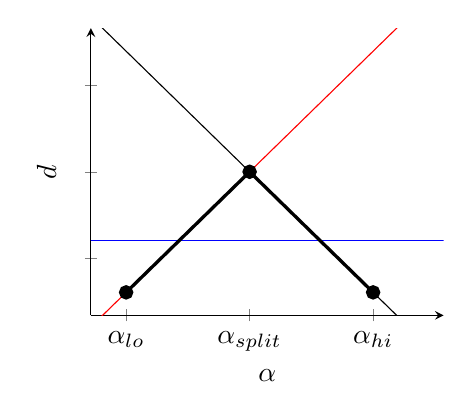
\begin{tikzpicture}
        \begin{axis}[ 
        axis x line=bottom,% only show the bottom x axis
        axis y line=left,
        xlabel=$\alpha$,
        ylabel={$d$},
        xmin=0.4,
        xmax=0.9,
        xtick={0.45,0.625,0.8},
        xticklabels={$\alpha_{lo}$, $\alpha_{split}$, $\alpha_{hi}$},
        width=0.5\textwidth,
        yticklabels={,,}
        ] 
        
        \addplot[mark=none, red] {-3+8*x}; 
        \addplot[mark=none, black] {-8*x+7};
        \addplot[mark=none, blue] {1.2};
        \addplot [mark=*,very thick] table {
        0.45   0.6
        0.625  2
        0.8    0.6
        };
        \end{axis} 
    \end{tikzpicture}
    \caption{Simply calculating the split values between the start and the end value of the range $[\alpha_{lo}, \alpha_{hi}]$ will not necessarily lead to the optimal values. By doing so, the blue line (constant $d$ value) will not be considered.}
    \label{fig:notoptimal}
\end{figure}

In order to solve this, we can recursively check each resulting interval again if it contains different merging behaviors, i.e.\ we check the behaviors for both $\alo$ and $\ahi$ to find a value $\alpha_{split}$ and afterwards do the same check for the new intervals $[\alo, \alpha_{split})$ and $[\alpha_{split}, \ahi)$. We repeat this approach recursively until the merges for each of the subintervals' limits $\alo$ and $\ahi$ agree, because we then know that there is no linear function that we did not discover.

\begin{figure}[H]
    \centering
    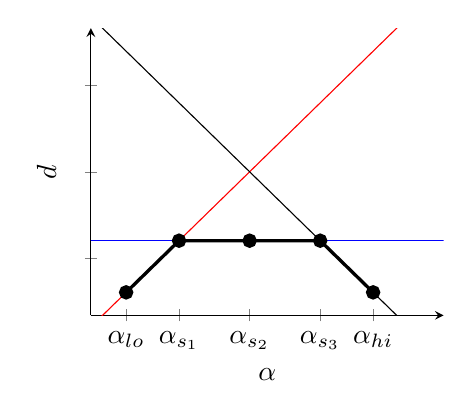
\begin{tikzpicture}
        \begin{axis}[ 
        axis x line=bottom,% only show the bottom x axis
        axis y line=left,
        xlabel=$\alpha$,
        ylabel={$d$},
        xmin=0.4,
        xmax=0.9,
        xtick={0.45,0.525,0.625,0.725,0.8},
        xticklabels={$\alpha_{lo}$, $\alpha_{s_1}$, $\alpha_{s_2}$, $\alpha_{s_3}$, $\alpha_{hi}$},
        width=0.5\textwidth,
        yticklabels={,,}
        ] 
        \addplot[mark=none, red] {-3+8*x}; 
        \addplot[mark=none, black] {-8*x+7};
        \addplot[mark=none, blue] {1.2};
        \addplot [mark=*,very thick] table {
        0.45   0.6
        0.525  1.2
        0.625  1.2
        0.725  1.2
        0.8    0.6
        };
        \end{axis} 
    \end{tikzpicture}
    \caption{Calculating the split values between the start and the end value of the range $[\alpha_{lo}, \alpha_{hi}]$ recursively will lead to the optimal values, however it results in one unnecessary interval in the given example.}
    \label{fig:notoptimal2}
\end{figure}

By calculating the split points recursively, the example in figure \ref{fig:notoptimal2} will result in the intervals $[\alpha_{lo}, \alpha_{s_1})$, $[\alpha_{s_1}, \alpha_{s_2})$, $[\alpha_{s_2}, \alpha_{s_3})$ and $[\alpha_{s_3}, \alpha_{hi})$. The optimal distance between $\alpha_{s_1}$ and $\alpha_{s_3}$ is covered now, but the results contain one unnecessary interval as $\alpha_{s_2}$ still divides two intervals. The algorithm can check if older splits are still relevant, however the runtime cost to do so will be more expensive than carrying one additional interval with the same distance. We can use this knowledge and adapt algorithm \ref{alg:alphalinkage1}.

\begin{algorithm}
    \textbf{Input:} Merge functions $\DZero$ and $\DOne$, clustering instance $S = \{x_1, \dots, x_n\}$ and initial state $st$
    \begin{enumerate}[nosep, leftmargin=*]
    \item Let $\mathcal{I} = \emptyset$ be the initially empty set of parameter intervals.
    \item For iteration $1$ : $n-1$
    \begin{itemize}[nosep, leftmargin=*]
        \item For each state $s \in st$
        \begin{enumerate}[nosep, leftmargin=*]
            \item remove state $s$
            \item ranges $\gets$ find ranges between $s.\alo$ and $s.\ahi$
            \item For each range $r \in$ ranges
            \begin{enumerate}
                \item $A, B \gets$ candidate for range
                \item $ms \gets$ merge $A, B$\;
                \item add state $ms$ with range $r$ to the end of $st$
            \end{enumerate}
        \end{enumerate}
    \end{itemize}
    \item For output state $s \in st$
            \begin{itemize}
                \item add interval $i = [s.\alo, s.\ahi)$ to $\mathcal{I}$
            \end{itemize}
        \item Return $\mathcal{I}$
    \end{enumerate}
    \caption{Recursive Interval Calculation}
    \label{alg:alphalinkage2}
\end{algorithm}

As experimental results turn out to need a lot of memory (up to $\approx$ 2 GB for 300 points and 20,000 states), we want to adapt algorithm \ref{alg:alphalinkage2} so that it uses less memory. The memory usage scales relative to the amount of currently in-memory stored states, so the goal is to reduce these. As the amount of states is much larger than the amound of iterations, we calculate and evaluate the leave nodes of the tree and keep the alternative merges stored, i.e.\ we use a depth-first instead of a breadth-first approach. This results in algorithm \ref{alg:alphalinkage3}.

\begin{algorithm}
    \textbf{Input:} Merge functions $\DZero$ and $\DOne$, clustering instance $S = \{x_1, \dots, x_n\}$ and initial state $st$
    \begin{enumerate}[nosep, leftmargin=*]
    \item Let $\mathcal{I} = \emptyset$ be the initially empty set of parameter intervals.
    \item While $|st| > 0$
    \begin{itemize}[nosep, leftmargin=*]
        \item For each state $s \in st$
        \begin{enumerate}
            \item remove state $s$\;
            \item If $s$ is final: add interval $i = [s.\alo, s.\ahi)$ to $\mathcal{I}$
            \item Else: 
            \begin{enumerate}
                \item ranges $\gets$ find ranges between $s.\alpha_{lo}$ and $s.\alpha_{hi}$
                \item For each range $r \in ranges$
                \begin{enumerate}
                    \item $A, B \gets$ candidate for range
                    \item $ms \gets$ merge $A, B$
                    \item add state $ms$ with range $r$ to the beginning of $st$
                \end{enumerate}
            \end{enumerate}
        \end{enumerate}
    \end{itemize}
    \item Return $\mathcal{I}$
    \end{enumerate}
    \caption{Depth-first $\alpha$-linkage}
    \label{alg:alphalinkage3}
\end{algorithm}

Using a depth-first implementation instead of a breadth-first implementation leads to huge benefits. We do not need a lot of memory anymore and together with the memory / copying costs, we also improve the runtime. Figure \ref{fig:performance} gives insights about the memory usage and the required runtime for our MNIST experiments with algorithm \ref{alg:alphalinkage2} (breadth-first) and algorithm \ref{alg:alphalinkage3} (depth-first). We notice that the memory usage for the breadth-first implementation had an exponential growth. Clustering 500 points already needed 8 GB of memory, that was the maximum of the device the experiments were run on, i.e.\ for larger-scale experiments we would have been forced to use better hardware. Instead, with the depth-first implementation we have a linear growth over the points and it is possible to reduce the amount of needed memory further if the intervals do not have to be stored in-memory, e.g.\ when we run an experiment on one dataset, we can directly export resulting intervals. For the breadth-first approach this would also be possible, but not prior to the last iteration, as we have to store each interval in each of the previous iterations. In addition, figure \ref{fig:performance} shows that the runtime also benefits from using the depth-first implementation. While we needed more than one hour to evaluate 500 points, we now need less than 10 minutes. This allows us to scale up our experiments from so far $\approx 500$ points to $\approx 1,000$ points.

\begin{figure}
\centering
\begin{minipage}{.45\textwidth}
  \centering
  \includegraphics[width=\linewidth]{plots/memory_mnist_ac}
\end{minipage}\hfill
\begin{minipage}{.45\textwidth}
  \centering
  \includegraphics[width=\linewidth]{plots/runtime_mnist_ac}
\end{minipage}
\caption{The depth first implementation needs less memory and also has a better runtime compared to the breadth first implementation.}
\label{fig:performance}
\end{figure}

As an addition, instead of merging iteratively and steadily shrinking the intervals, we propose a tweaked version of algorithm \ref{alg:alphalinkage3} with a geometric motivation. We are again evaluating an interval $[\alpha_{lo}, \alpha_{hi}]$, but we interpret the different merges as linear functions depending on $\alpha$. We start by calculating the merge candidate for the start value $\alpha_{lo}$ and calculate the next intersection that will yield to the next merge. By calculating all the intersections of linear functions, we can also determine all the different intervals for the range $[\alpha_{lo}, \alpha_{hi}]$, where different merging behaviors occur. Algorithm \ref{alg:alphalinkage4} describes this procedure.

\begin{algorithm}
    \textbf{Input:} Merge functions $\DZero$ and $\DOne$, clustering instance $S = \{x_1, \dots, x_n\}$ and initial state $st$
    \begin{enumerate}[nosep, leftmargin=*]
    \item Let $\mathcal{I} = \emptyset$ be the initially empty set of parameter intervals.
    \item While $|st| > 0$
    \begin{itemize}[nosep, leftmargin=*]
        \item For each state $s \in st$
        \begin{enumerate}
            \item remove state $s$\;
            \item If $s$ is final: add interval $i = [s.\alo, s.\ahi)$ to $\mathcal{I}$
            \item Else: 
            \begin{enumerate}
                \item $\alpha \gets \alpha_{lo}$\;
                \item linear function $lf \gets$ get lf for $\alpha$
                \item While $\alpha < \alpha_{hi}$
                \begin{enumerate}
                    \item $\alpha_{new} \gets$ calculate next split for $\alpha$
                    \item $lf \gets$ get lf for $\alpha_{new}$\;
                    \item $\alpha \gets \alpha_{new}$
                \end{enumerate}
            \end{enumerate}
        \end{enumerate}
    \end{itemize}
    \item Return $\mathcal{I}$
    \end{enumerate}
    \caption{$\alpha$-linkage with Geometric Interval Calculation}
    \label{alg:alphalinkage4}
\end{algorithm}

Algorithm \ref{alg:alphalinkage4} runs once for each merge, leading to $M$ iterations. In each iteration, we find the closest pair of clusters according to $D_\alpha$ using $O(m^2)$ evaluations of the merge functions $D_0$ and $D_1$. We add the cost of evaluating $D_0$ and $D_1$ with K leading to the total runtime of $O(Mm^2K)$. This leads to a clean implementation, where we do not store unnecessary intervals (see figure \ref{fig:notoptimal2}) any longer. In contrast, we now only store the intervals where different merges occur. By interpreting the geometrics of linear functions, we always find the optimal merges for any value of $\alpha$ leading to well-defined intervals for any clustering instance interpolating within $\dsc$, $\dsa$ or $\dac$. Figure \ref{fig:optimal} shows the optimized merge selection of the exemplary distance functions.

\begin{figure}
    \centering
    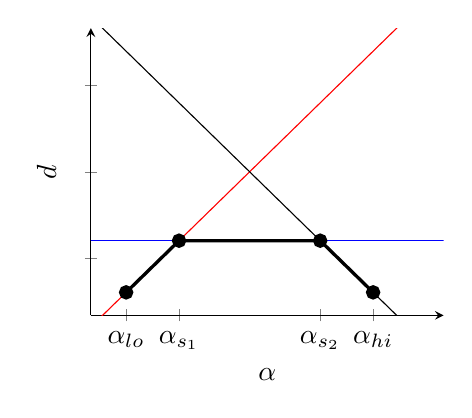
\begin{tikzpicture}
        \begin{axis}[ 
        axis x line=bottom,% only show the bottom x axis
        axis y line=left,
        xlabel=$\alpha$,
        ylabel={$d$},
        xmin=0.4,
        xmax=0.9,
        xtick={0.45,0.525,0.725,0.8},
        xticklabels={$\alpha_{lo}$, $\alpha_{s_1}$, $\alpha_{s_2}$, $\alpha_{hi}$},
        width=0.5\textwidth,
        yticklabels={,,}
        ] 
        \addplot[mark=none, red] {-3+8*x}; 
        \addplot[mark=none, black] {-8*x+7};
        \addplot[mark=none, blue] {1.2};
        \addplot [mark=*,very thick] table {
        0.45   0.6
        0.525  1.2
        0.725  1.2
        0.8    0.6
        };
        \end{axis} 
    \end{tikzpicture}
    \caption{Geometrically calculating the split points between the linear distance functions leads to the optimal results and does not store unnecessary intervals.}
    \label{fig:optimal}
\end{figure}

\section{Performance Optimizations}

In order to have real-world applications, the proposed algorithms should run in an efficient way, i.e.\ it should not take the $\alpha$-linkage algorithms too much time to run. A first python implementation took days to run, but switching to C++ and using its advantages took down the runtime to hours for large-scale experiments. However, there are more optimization methods that we used in order to improve the runtime.

\subsection{Dynamic Programming}

One of the most time-consuming parts was the calculation of the distances. For each pair of clusters $C_i, C_j$ the distance had to be calculated for each clustering state. We optimized this by using dynamic programming to store the distance matrices $D_{lower}$ and $D_{upper}$ for each state. We interpolate from one linkage distance (lower) to another linkage distance (upper), e.g.\ the $\dsc$ setting describes the interpolation from single linkage (lower) to complete linkage (upper). In this example we then store the pairwise distances for both single linkage and complete linkage and in order to find the merge candidates we have to iterate over the distance matrices instead of calculating the distances redundantly. When we merge two clusters, we then update the distance matrices for the given state. Table \ref{dp:distances} shows an example for the pairwise distances of clusters $i$ and $j$. One observation that we can make is that the matrix has a lot of redundant values, because all our distance functions are symmetric, i.e.\ $D(i,j) = D(j,i)$. Removing these redundant values will result in a trade-off between copying and indexing costs and will be discussed in the following section. Another optimization we can do is to store the indices of the active clusters, i.e.\ the clusters that can get merged. Once two clusters got merged, they cannot be merged any further, only the resulting cluster can. So we then do not have to consider the old clusters anymore and can remove them from the set of active indices. This allows us to find the merge candidates faster as the pool of candidates gets smaller over time.

\begin{table}[H]
    \centering
    \begin{tabular}{|l | l l l l l|}
    \hline
    j\textbackslash i & 0 & 1 & 2 & 3 & 4\\ \hline
    0 & 0 & 1.243 & 1.512 & 2.468 & 5.1243\\
    1 & 1.243 & 0 & 2.443 & 3.1412 & 4.443\\
    2 & 1.512 & 2.443 & 0 & 3.8988 & 6.827\\
    3 & 2.468 & 3.1412 & 3.8988 & 0 & 5.72\\
    4 & 5.1243 & 4.443 & 6.827 & 5.72 & 0\\ \hline
    \end{tabular}
    \caption{Storing the pairwise distances of all clusters avoids calculating the distances redundantly.}
    \label{dp:distances}
\end{table}

\subsection{Trade-Off between Copying and Indexing Costs}

Currently we can access the costs for a pair of clusters $C_i$ and $C_j$ through $D[i,j]$ or $D[i + j * width]$ for flattened matrices. These indices are very easy to determine. In order to remove the redundant values from the distance matrix we remove all values below the diagonal as shown in table \ref{dp:distances2}.

\begin{table}[h]
    \centering
    \begin{tabular}{|l | l l l l l|}
    \hline
    j\textbackslash i & 0 & 1 & 2 & 3 & 4\\ \hline
    0 & 0 & 1.243 & 1.512 & 2.468 & 5.1243\\
    1 & \cellcolor{gray!25} & 0 & 2.443 & 3.1412 & 4.443\\
    2 & \cellcolor{gray!25} & \cellcolor{gray!25} & 0 & 3.8988 & 6.827\\
    3 & \cellcolor{gray!25} & \cellcolor{gray!25} & \cellcolor{gray!25} & 0 & 5.72\\
    4 & \cellcolor{gray!25} & \cellcolor{gray!25} & \cellcolor{gray!25} & \cellcolor{gray!25} & 0\\ \hline
    \end{tabular}
    \caption{Removing the redundant distance values leads to less memory usage, but to more complex index calculations.}
    \label{dp:distances2}
\end{table}

In addition, we can also remove the diagonal values as they represent the distances between the same clusters ($D(i,i)$) and are thus always zero. This results in table \ref{dp:distances3}.

\begin{table}[H]
    \centering
    \begin{tabular}{|l | l l l l l|}
    \hline
    j\textbackslash i & 0 & 1 & 2 & 3 & 4\\ \hline
    0 & \cellcolor{gray!25} & 1.243 & 1.512 & 2.468 & 5.1243\\
    1 & \cellcolor{gray!25} & \cellcolor{gray!25} & 2.443 & 3.1412 & 4.443\\
    2 & \cellcolor{gray!25} & \cellcolor{gray!25} & \cellcolor{gray!25} & 3.8988 & 6.827\\
    3 & \cellcolor{gray!25} & \cellcolor{gray!25} & \cellcolor{gray!25} & \cellcolor{gray!25} & 5.72\\
    4 & \cellcolor{gray!25} & \cellcolor{gray!25} & \cellcolor{gray!25} & \cellcolor{gray!25} & \cellcolor{gray!25} \\ \hline
    \end{tabular}
    \caption{We also get rid of the distances between the same clusters in the stored distance matrices.}
    \label{dp:distances3}
\end{table}

The matrices are now smaller, so they need less memory. In the example, we changed a matrix of the size $25$ to a matrix of the size $10$. In general, a matrix of the size $n \times n$ will be compressed to a matrix of the size $\frac{n^2-n}{2}$. The lower amount of needed memory also results in less copying costs that will lead to a better runtime. However, the indexing is not as trivial anymore. For easier storage, we again work with flattened matrices, the indexing for the resulting list is shown in equation \ref{eq:indexing}.

\begin{equation}
    \begin{aligned}
        index(i,j) = \frac{width * (width - 1)}{2} - \frac{(width - j) * (width - j - 1)}{2} + i - j - 1
    \end{aligned}
    \label{eq:indexing}
\end{equation}

Calculating this index in a nested loop is very expensive, however we calculate the part $index(j)$ that does not depend on $i$ in the outer loop and thus only need to add $i$ in the inner loop. This does not only yield to a lower memory usage of $\approx 30\%$, but also increases the runtime by roughly the same factor.

\subsection{Implementation-specific Optimizations}

In order to optimize the implementation even further, we will have a look into the implementation. One optimization that already was briefly described is the flatterning of the matrices, so the resulting list will be one-dimensional and can be iterated easier.\\

Another observation is that copy operations are computationally expensive, so we avoid them as much as possible. In the described algorithms (\ref{alg:alphalinkage1}, \ref{alg:alphalinkage2}, \ref{alg:alphalinkage3} and \ref{alg:alphalinkage4}) we removed a state from the list of states and added other states. In an optimized way, we do not remove the state and just overwrite the state with the resulting state. Once there are splits in the current interval, the state gets overwritten and additional states get added to the list.\\

We can also optimize the way of updating the distance matrices. Instead of adding new clusters there for a merge of clusters $i$ and $j$ we update the distances of $i$ to all active clusters with the distances of the resulting cluster. The distances of the cluster $j$ will not be considered for merges anymore as the index $j$ gets removed from the active indices. This has the advantage that the size of the distance matrices will not increase after merges.\\

Also, the data types make an important contribution to the memory usage. Instead of using double precision floating point values, single precision is enough to clearly identify and separate all the resulting intervals. Same goes for the distances as we only need the minimum and maximum distances, that are not effected by loss of precision. To store the indices of the clusters, we know that our experiments will not exceed $2^{16}$ points, so they can be stored as half precision values.